
%
%  $Description: Author guidelines and sample document in LaTeX 2.09$
%
%  $Author: ienne $
%  $Date: 1995/09/15 15:20:59 $
%  $Revision: 1.4 $
%

\documentclass[times, 10pt,twocolumn]{article}
\usepackage{latex8}
\usepackage{times}
%my packages:
\usepackage{graphicx}
\usepackage{amsmath}
\usepackage{amssymb}
\usepackage{flushend}

%\documentstyle[times,art10,twocolumn,latex8]{article}

%-------------------------------------------------------------------------
% take the % away on next line to produce the final camera-ready version
\pagestyle{empty}

%-------------------------------------------------------------------------
\begin{document}

\title{SMT-based Test Program Generation for Cache-memory Testing}

\author{Evgeni Kornikhin\\
Institute for System Programming of RAS\\ Solzhenitsyn St., 25,
Moscow, Russia\\ kornevgen@ispras.ru\\
}

\maketitle
\thispagestyle{empty}

\begin{abstract}
Core-level verification of microprocessors is performed using many
assembly programs (test programs). Instructions (and their behavior)
for test program can be selected combinatorially. But special
initial values for registers are required to satisfy this test
program. This article proposes algorithm for generation these
values. The article considers instructions performed memory access
through cache. Proposing algorithm describes test program behavior
as SMT-assertions and uses SMT-solvers to get initial values of
registers for given initial state of cache-memory. Algorithm is
presented for LRU cache memory, but the same ideas are applicable
for other displacing policies.
\end{abstract}



\section{Introduction}

System functional testing of microprocessors uses many assembly
programs (\emph{test programs}). Such programs are loaded to the
memory, executed, execution process is logged and analyzed. But
modern processors testing requires a lot of test programs. Technical
way of test program generation was proposed in~\cite{kamkin}. This
way based on the microprocessor's model. Its first stage is
systematic generation abstract test programs (\emph{test
templates}). This abstract form contains a sequence of instructions
with arguments (registers) and \emph{test situations} (behavior of
this instruction; these can be overflow, cache hits, cache misses).
The second stage is generation of initial microprocessor state for
given test template, i.e. initial values of registers. Technical way
from~\cite{kamkin} is useful for aimed testing when aim is expressed
by instruction sequence with specific behavior. Based on registers
values the third, final, stage is generation the sequence of
instructions to reach initial microprocessor state. This sequence of
instructions with test template get ready assembly program. This
paper devoted to the second stage, i.e. initial state generation.

Known researches about test data generation problem contain the
following methods of its solving:
\begin{enumerate}
\item combinatorial methods;
\item ATPG-based methods;
\item constraint-based methods.
\end{enumerate}

Combinatorial methods are useful for simple test templates (each
variable has explicit directive of its domain, each value in domain
is possess)~\cite{combinatorial}. ATPG-based methods are useful for
structural but not functional testing~\cite{ATPG}. Constraint-based
methods are the most promising methods. Test template is translated
to the set of constraints (predicates) with variables which
represented test data. Then special solver generates values for
variables to satisfy all constraints. This paper contains
constraint-based method also. IBM uses constraint-based method in
Genesys-Pro~\cite{GenesysPro}. But it works inefficiently on test
templates from~\cite{kamkin}. Authors of another constraint-based
methods restrict on registers only and don't consider cache-memory.

\section{Preliminaries}

\subsection{Test templates description}

Test template defines requirements to the future test program. Test
template contains sequence of instructions. Each element of this
sequence has instruction name, arguments (registers, addresses,
values) and \emph{test situation} (constraint on values of arguments and
microprocessor state before execution of instruction). Example of
test template description for model instruction set:

REGISTER reg1 : 64;

REGISTER reg2 : 64;

LOAD reg1, reg2 @ l1Miss

STORE reg2, reg1 @ l1Hit

This template has 2 instructions -- LOAD and STORE. Template begins
from variable definitions (consist of name and bit-length). Test
situation is specified after "@": test situation of the first
instruction if "l1Hit" (which means hit in first-level cache) and
test situation of the second instruction is "l1Miss" (which means
miss in first-level cache).

\begin{itemize}
\item "LOAD reg1, reg2" loads value from memory by \emph{virtual}
address from register "reg2" to the register "reg1";
\item "STORE reg1, reg2" stores value from register "reg1" to the
memory by \emph{virtual} address in "reg2".
\end{itemize}

The article considers full memory access only. Otherwords, behavior
of "LOAD/STORE x, y" is the following: the first step is physical
address generation (\emph{address translation}) and the second step
is memory access through cache using generated physical address (see
pic.~\ref{LOAD}).

\begin{figure}[h]\label{LOAD}
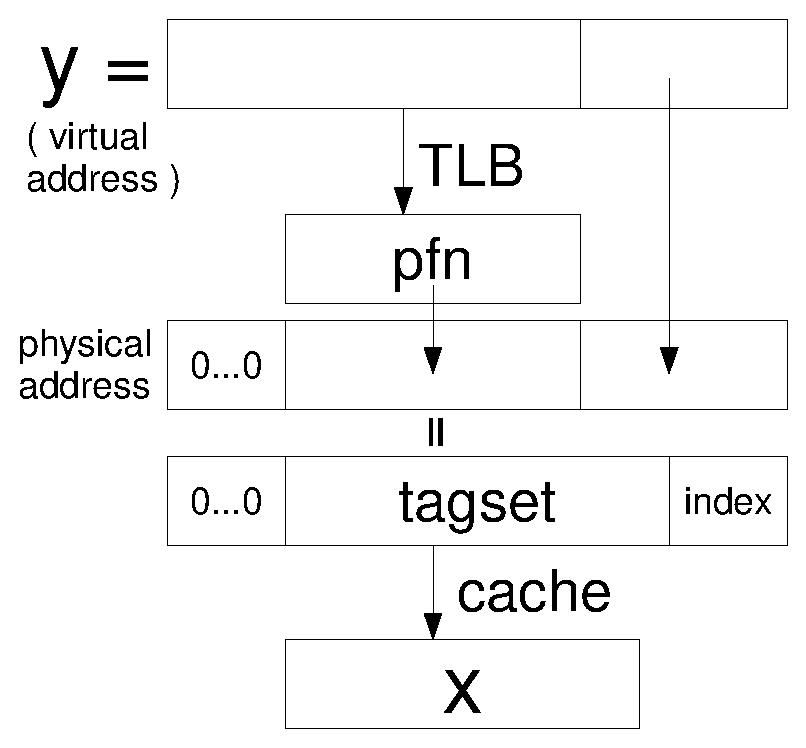
\includegraphics[width=0.4\textwidth]{load}
\caption{Model of LOAD/STORE instructions.}
\end{figure} %\\ \noindent

\subsection{Tagsets}

Cache access is based on physical address tag. It is compared with
tags of cached data from all sections by index from physical
address. Tag and index is a bit-field of physical address. Term
\emph{tagset} will be a bit-concatenation of tag and index (see
pic.~\ref{LOAD}). Each LOAD/STORE instruction has a tagset.

Physical address is arranged from physical frame number (pfn) and
offset in page (see pic.~\ref{LOAD}). So pfn is a bit-field of
physical address. Tagset is a bit-field of physical address also.
Lets denote $x_{<\mbox{pfn bits}>}$ bits of tagset $x$ which are
included in pfn. Lets denote $x_{<\mbox{index bits}>}$ bits of
tagset $x$ which are included in index bit-field.

\subsection{Satisfiability Modulo Theories}
SMT (Satisfiability Modulo Theories) problem is "the satisfiability
problem of the quantifier-free fragment of various first-order
theories"~\cite{SMT}. SMT-solvers concern SMT problem as SAT problem
(satisfiability) with special terms. Conjunctions of these terms can
be satisfied by special algorithms and heuristics. Examples of
SMT-solvers are Yices~\cite{Yices}, Z3~\cite{Z3}, CVC3~\cite{CVC3}.
This article uses bit-vector theory for constraints described
tagsets and registers values relations.

\subsection{Limitations of the approach}
There are some requirements to the testing process which are took
into account and efficiently used in proposing approach.
\begin{enumerate}
\item known initial state of the cache and TLB; this is a key
requirement of the approach; initial state is used for initial
values of registers generation;
\item hits in Joint TLB are considered only; misses (i.e., absence a
TLB line for virtual address) requires hardware or software
refilling programs, so this test situations are very hard for
constraints definition;
\item address translation and cache access are required for each
memory access instruction (i.e., proposed method works for `Cached
Mapped' segments of virtual memory only; another segments may
require more complex constraints because of number of cases growth);
\item non-unified cache (otherwords, either data cache only, or
instruction cache only);
\item non-VIVT cache (virtually tagged, virtually indexed~\cite{memory_systems}).
\end{enumerate}

\section{Test case generation}

Test case is a test program. Each test program consists of
initialization instructions, body instructions and finalization
instructions. Initialization instruction prepare microprocessor to
the appropriate state. Then body instructions are executed (they are
defined in test template). And finalization instructions check state
of microprocessor after body instructions execution (for example,
check values for registers). Given test template contains required
instructions sequence and hit/misses sequence. These instructions
become body instructions. The proposing algorithm generated
initialization instructions according to hit/miss sequence.

The aim of proposing algorithm is generation initial values for
registers using solution of SMT-constraints. Generated initial
values are used for initialization instructions generation.
SMT-constraints describe relations on registers values. Each
instruction can change values of registers and cache
state.

New variables are introduced to describe changes of cache state.
These variables are tagsets. They don't present cache as it is (by
cells). Instead of this constraints on tagsets describe relations
between virtual addresses of instructions. Tagsets are used to
describe hit/miss sequence. Registers are used to get virtual
addresses (as second arguments of LOAD and STORE) and values loaded
or stored to memory (as first arguments of LOAD and STORE).

The following constraints present cache behavior for test templates
with no more than $w$ instructions (although method works for any
test templates). $w$ is associativity of cache.

\subsection{Tagsets constraints}

Lets use "hit($x$)" and "miss($x$)" as test situation for
instruction ($x$ is a tagset). Lets $L$ is set of all tagsets from
initial cache state and $PFN$ is set of all physical frame number
fields of TLB lines from initial TLB state. Lets $LP = \{ x | x \in
L \wedge x_{<\mbox{pfn~bits}>} \in PFN\}$.

"hit($x$)" can be presented as the following disjunction: "Either
$x$ was in the initial state and hasn't been displaced, or $x$ has
been added to the cache by cache miss". If $x$ was in the initial
state and it is not occurred yet, then there are \emph{non many}
instructions which help to displace $x$. "Non many" means no more
than $w-\delta$, when $w$ is cache associativity, $\delta$ is
lru-counter of $x$ ($x \in LP$, so $LP$ can be searched as $x =
\lambda_\delta, \lambda_\delta \in LP$), $1 \leqslant \delta
\leqslant w$ ($\delta=1$ is counter of the youngest tag, $\delta=w$
is counter of the oldest tag).

"miss($x$)" can be presented as the following disjunction: "Either
$x$ is not occurred yet, or $x$ was in the initial state and has
been displaced already". If $x$ was in the initial state and it has
been displaced already, then there are \emph{many} instructions
which help to displace $x$. "Many" means more than $w-\delta$, when
$w$ is cache associativity, $\delta$ is lru-counter of $x$ ($x \in
LP$, so $LP$ can be searched as $x = \lambda_\delta, \lambda_\delta
\in LP$).

It is enough to express this logic using SMT-constraints. So the
following constraints are added for each "hit($x$)" ($x_1, x_2, ...,
x_n$ are all tagsets of previous instructions):
$$\left[\begin{array}{l}
x\in\{x_1, x_2, ..., x_n\}\\
\bigvee\limits_{\lambda_\delta \in LP} (x = \lambda_\delta \wedge
\sum\limits_{i=1}^n u_x(x_i) \leqslant w - \delta)\\
\end{array}\right.$$

$u_x: \mbox{tagset} \rightarrow \{0, 1\}$ is \mbox{usefulness
function}. It equals 1 for tagset which helps to displace $x$ and
equals 0 for tagset which doesn't help to displace $x$. Usefulness
function has the following representation using SMT-constraints:
$$u_x(x_i) \equiv \left\{\begin{array}{l}
x_i\in\{\lambda_{\delta+1}, ..., \lambda_w\}~\wedge\\
\qquad x_i\notin\{x_1, ..., x_{i-1}\}, \mbox{if}~x_i~\mbox{gets hit}\\
{x_i}_{<\mbox{index bits}>} = {x}_{<\mbox{index bits}>}, \mbox{if}~x_i~\mbox{gets miss}\\
\end{array}\right.$$

And the following constraints for "miss($x$)" ($x_1, x_2, ..., x_n$
are all tagsets of previous instructions):
$$\left[\begin{array}{l}
x\notin LP \wedge x\notin\{x_1, x_2, ..., x_n\}\\
\bigvee\limits_{\lambda_\delta \in LP} (x = \lambda_\delta \wedge x
\notin \{x_1, ..., x_n\} \wedge
\sum\limits_{i=1}^n u_x(x_i) > w - \delta)\\
\end{array}\right.$$

These constraints describe cache behavior without exponential
selection all values of any variable. And often $LP$ is not large.
Proposed algorithm is correct, full and defines fast way to get
values of tagsets.

\subsection{Register constraints}

Tagsets are useful to describe "hit/miss" sequence but aim is
generation of initial register values. Tagsets depend on register
values (because register values get virtual addresses) and register
values depend on tagsets (because data from memory corresponds to
physical address). These dependencies must be represented as
constraints and added to the final constraints system for
SMT-solver. Additional constraints describe address translation
(1-3) and memory access(4-5):
\begin{enumerate}

\item low bits of tagset equal to the high bits of virtual address's offset for each
instruction "LOAD/STORE $x, y$" with tagset $ts$;

\item high bits of virtual address correspond to high bits of tagset
(physical frame number bits) for each instruction "LOAD/STORE $x,
y$" with tagset $ts$; these constraints depend on TLB structure;

\item high bits of virtual address correspond to the segment of
virtual memory (virtual memory space -- some virtual addresses can
be mapped or can't be mapped, can be cached or can't be cached);

\item for each pair "STORE $x_1, y_1$"
and "LOAD $x_2, y_2$" (LOAD follows from STORE) $phys_1 = phys_2
\wedge phys_1 \notin P \rightarrow x_1 = x_2$, where $phys_1$ and
$phys_2$ are physical addresses, $P$ is a set of physical addresses
of STORE instructions between these "STORE" and "LOAD" instructions;

\item for each pair "LOAD
$x_1, y_1$" and "LOAD $x_2, y_2$" (the second LOAD follows from the
first LOAD) $phys_1 = phys_2 \wedge phys_1 \notin P \rightarrow x_1
= x_2$, where $phys_1$ and $phys_2$ are physical addresses, $P$ is
set of physical addresses of STORE instructions between these "LOAD"
instructions.
\end{enumerate}

\subsection{SMT representation of constraints}
All generated constraints can be (and should be) represented by
constraints by QF\_BV logic~\cite{smt-lib} (bit-vectors with
bit-extraction operation and equality relation) and efficiently
solved by SMT-solver (we use Z3).

\section{Conclusions}
The article has presented the algorithm for generation test programs
used in cache-memory testing. It generates constraints on initial
register values and some additional variables efficiently. These
constraints can be solved efficiently by ordinary SMT-solver (for
example, Z3).

The algorithm has been presented for LRU physically tagged
physically indexed set-associative cache-memory and test templates
with no more than $w$ instructions. Further it is planned to
increase the algorithm for test situations with uncached or unmapped
access and add possibility to offer changes of cache-memory before
test program execution to cover more test templates.

%\phantomsection
\renewcommand{\refname}{5 ~~ References}

\bibliographystyle{latex8}
\bibliography{ksmt}

\end{document}
